%!TeX root=../monografia.tex

%% ------------------------------------------------------------------------- %%
\chapter{Link-Cut Trees}
\label{cap:link-cut-trees}

Neste capítulo, apresentaremos as \emph{link-cut trees}, introduzida por ~\citet{10.1145/800076.802464}. Esta estrutura de dados serve como base para as estruturas retroativas apresentadas nos próximos capítulos.

%% ------------------------------------------------------------------------- %%
\section{Ideia}
\label{sec:lct-ideia}

As link-cut trees são uma estrutura de dados que nos permite manter uma floresta de árvores enraizadas com peso nas arestas, onde os vértices de cada árvore possuem um número arbitrário de filhos. Ademais, a floresta armazenada por essa estrutura não é orientada --- isto é, suas arestas não possuem uma direção --- e devido à maneira que ela é usada nas implementações a seguir, sua raiz é constantemente redefinida, de modo que perdemos o arranjo original das árvores. Com isso, essa estrutura nos fornece o seguinte conjunto de operações:

\begin{itemize}
    \item \texttt{make\_root(u)}: enraíza no vértice $u$ a árvore que o contém.
    \item \texttt{link(u, v, w)}: dado que os vértices $u$ e $v$ estão em árvores separadas, transforma $v$ em raiz de sua árvore e o liga como filho de $u$, colocando peso $w$ na nova aresta criada.
    \item \texttt{cut(u, v)}: retira da floresta a aresta com pontas em $u$ e $v$, quebrando a árvore que continha estes vértices em duas novas árvores.
    \item \texttt{is\_connected(u, v)}: retorna \texttt{verdadeiro} caso $u$ e $v$ pertençam à mesma árvore, \texttt{falso} caso contrário.
\end{itemize}

Por último, as link-cut trees possuem a capacidade de realizar operações agregadas nos vértices, isto é, consultas acerca de propriedades de uma sub-árvore ou de um caminho entre dois vértices. Em particular, estamos interessados na rotina \texttt{maximum\_edge(u, v)}, que nos informa o peso máximo de uma aresta no caminho entre os vértices $u$ e $v$.

Todas essas operações consomem tempo $\Oh(\log n)$ amortizado, onde $n$ é o número de vértices na floresta.

%% ------------------------------------------------------------------------- %%
\section{Definições}
\label{sec:lct-definicoes}

Primeiramente, precisamos apresentar algumas definições acerca da estrutura que vamos estudar.

Chamamos de \emph{árvores representadas} as componentes da floresta armazenada nas link-cut trees. Para a representação que as link-cut trees utilizam internamente, dividimos uma árvore representada em caminhos vértice-disjuntos, os chamados \emph{caminhos preferidos}. Todo caminho preferido vai de um vértice a um ancestral deste vértice na árvore representada. Por conveniência, definimos o início de um caminho preferido como o vértice mais profundo contido nele.

Se uma aresta faz parte de um caminho preferido, a chamamos de \emph{aresta preferida}. Ademais, mantemos a propriedade de que um vértice pode ter no máximo uma aresta preferida com a outra ponta em algum de seus filhos. Caso tal aresta exista, ela liga um vértice a seu \emph{filho preferido}.

Finalmente, para cada caminho preferido, elegemos um \emph{vértice identificador}. A manutenção deste vértice será importante para a estrutura auxiliar que utilizaremos para manter os caminhos preferidos, dado que o vértice identificador de um caminho preferido será responsável por guardar um ponteiro para um vértice da árvore imediatamente acima do caminho preferido.

Ademais, para armazenar os pesos das arestas da floresta, a estrutura usada terá nós para vértices e para arestas da floresta. O nó correspondente à aresta $uv$ tem o vértice $u$ como seu pai e $v$ como seu único filho, e armazena o peso de $uv$.

\begin{figure}
    \centering
    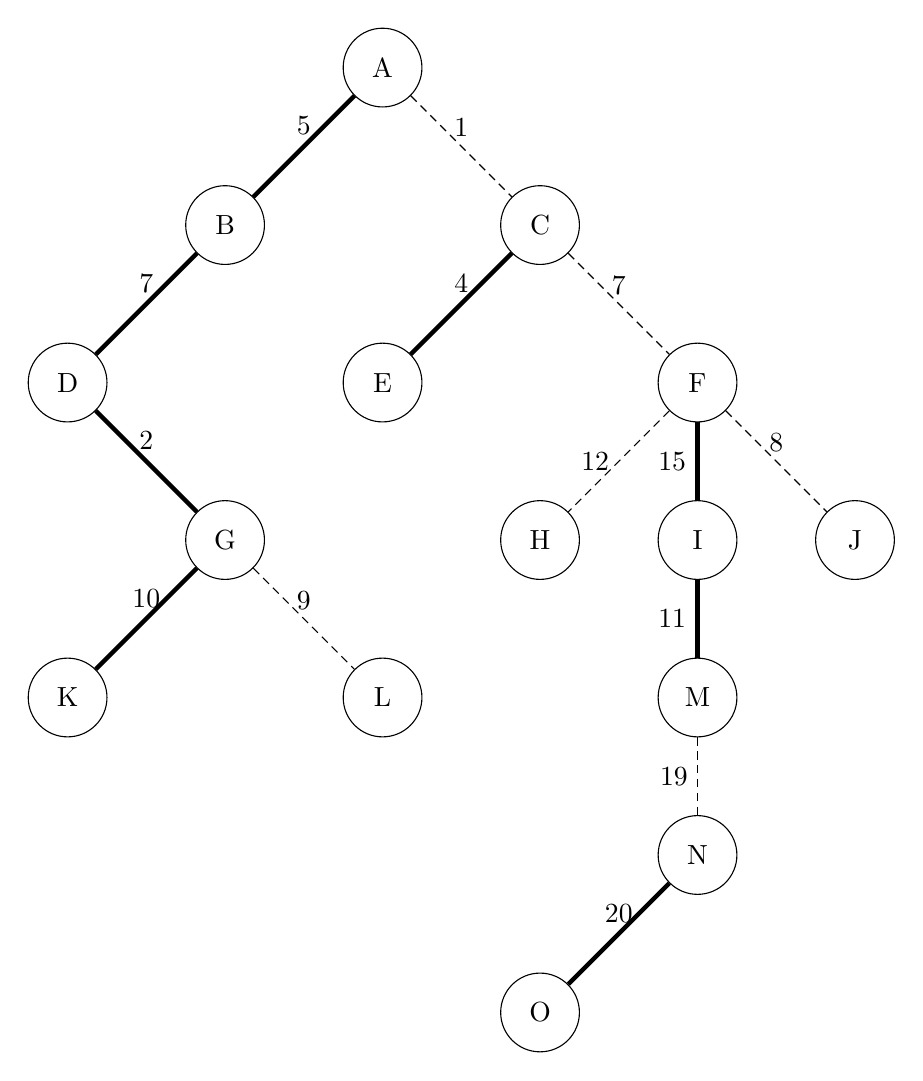
\begin{tikzpicture}[
            nointerno/.style={shape=circle, draw=black, minimum size=1cm},
            pref/.style={ultra thick},
            pptr/.style={densely dashed},
        ]
        \node[nointerno] (a) at (6, 20) {A};
        \node[nointerno] (b) at (4, 18) {B};
        \node[nointerno] (c) at (8, 18) {C};
        \node[nointerno] (d) at (2, 16) {D};
        \node[nointerno] (e) at (6, 16) {E};
        \node[nointerno] (f) at (10, 16) {F};
        \node[nointerno] (g) at (4, 14) {G};
        \node[nointerno] (h) at (8, 14) {H};
        \node[nointerno] (i) at (10, 14) {I};
        \node[nointerno] (j) at (12, 14) {J};
        \node[nointerno] (k) at (2, 12) {K};
        \node[nointerno] (l) at (6, 12) {L};
        \node[nointerno] (m) at (10, 12) {M};
        \node[nointerno] (n) at (10, 10) {N};
        \node[nointerno] (o) at (8, 8) {O};

        \draw[pref] (a) -- (b) node[midway, above] {5};
        \draw[pptr] (a) -- (c) node[midway, above] {1};
        \draw[pref] (b) -- (d) node[midway, above] {7};
        \draw[pref] (d) -- (g) node[midway, above] {2};
        \draw[pref] (g) -- (k) node[midway, above] {10};
        \draw[pptr] (g) -- (l) node[midway, above] {9};
        \draw[pptr] (c) -- (f) node[midway, above] {7};
        \draw[pref] (c) -- (e) node[midway, above] {4};
        \draw[pptr] (f) -- (h) node[midway, left] {12};
        \draw[pref] (f) -- (i) node[midway, left] {15};
        \draw[pptr] (f) -- (j) node[midway, above] {8};
        \draw[pref] (i) -- (m) node[midway, left] {11};
        \draw[pptr] (m) -- (n) node[midway, left] {19};
        \draw[pref] (n) -- (o) node[midway, above] {20};

    \end{tikzpicture}
    \caption{Árvore representada e seus caminhos preferidos. Na figura acima, as arestas escuras representam caminhos preferidos, com isso, temos o seguinte conjunto de caminhos vértice-disjuntos $ \{ \langle K,G,D,B,A \rangle, \langle E,C \rangle, \langle M,I,F \rangle, \langle L \rangle, \langle H \rangle, \langle J \rangle, \langle O,N \rangle \} $. }
    \label{fig:arvore-simples}
\end{figure}

%% ------------------------------------------------------------------------- %%
% access e como implementa o resto
\section{Operações}
\label{sec:lct-operacoes}

Nessa seção, apresentaremos o código por trás das operações que estamos interessados em implementar nas link-cut trees. Em um primeiro momento, assumiremos que já sabemos como implementar alguns métodos que lidam com os caminhos preferidos. Desta forma, a implementação dos métodos abaixo fica reservada para a próxima seção.

\begin{itemize}
    \item \texttt{make\_identifier(u)}: transforma um vértice $u$ em identificador de seu caminho preferido.
    \item \texttt{split(u)}: separa o caminho preferido em que o vértice $u$ é identificador em dois, quebrando a conexão entre $u$ e seu filho preferido, caso exista. Ao final, tanto $u$ quanto o seu filho preferido inicial serão os identificadores de seus caminhos preferidos.
    \item \texttt{join(u, v)}: recebe dois vértices, $u$ e $v$ --- identificadores de seus caminhos e sendo $v$ um filho de $u$ na árvore representada --- e concatena os respectivos caminhos preferidos, transformando $uv$ em aresta preferida de $u$. Com isso, separa $u$ da parte mais profunda de seu caminho preferido inicial, deixando o identificador de tal caminho com um ponteiro para $u$. Ao final da operação, $u$ será o identificador do novo caminho criado.
    \item \texttt{reverse\_path(u)}: recebe $u$, o identificador de um caminho preferido, e inverte a orientação desse caminho na árvore representada, isto é, o fim se transforma no começo e o começo no fim.
    \item \texttt{get\_path\_end\_node(u)}: retorna o vértice menos profundo do caminho preferido de $u$, em outras palavras, o vértice no fim do caminho preferido que contém $u$. Na árvore da Figura \ref{fig:arvore-simples}, a chamada \texttt{get\_path\_end\_node(G)} retorna o vértice \texttt{A}.
    \item \texttt{get\_parent\_path\_node(u)}: retorna o vértice na floresta imediatamente acima do fim do caminho preferido que contém $u$; no caso em que o caminho preferido de $u$ contém a raiz da árvore representada, este método retorna \texttt{null}. Na árvore da Figura \ref{fig:arvore-simples}, \texttt{get\_parent\_path\_node(M)} retorna o vértice \texttt{C} e \texttt{get\_parent\_path\_node(L)} retorna \texttt{G}.
    \item \texttt{get\_maximum\_path\_value(u)}: recebe $u$, o identificador de um caminho preferido, e retorna o maior valor de uma aresta neste caminho.
\end{itemize}

Além disso, de modo a determinarmos a complexidade dos métodos das link-cut trees, temos que \texttt{split}, \texttt{join}, \texttt{reverse\_path} e \texttt{get\_maximum\_path\_value} consomem tempo constante, enquanto \texttt{make\_identifier}, \texttt{get\_path\_end\_node} e \texttt{get\_parent\_path\_node} gastam tempo $\Oh(\log n)$ amortizado, onde $n$ é o número de vértices nos caminhos preferidos.

\subsection{Rotina Access}
\label{subsection:lct-access}

Uma rotina utilizada por todos os métodos das link-cut trees que vamos implementar é a \texttt{access}. A partir dela conseguimos reorganizar a estrutura interna de uma árvore representada a nosso favor. Basicamente, a operação \texttt{access(u)} cria um caminho preferido que parte de $u$ e vai até a raiz da árvore representada de $u$. Com isso, todas as arestas preferidas que tinham somente uma das pontas fazendo parte deste novo caminho deixam de ser preferidas e $u$ termina sem nenhum filho preferido.

Para isso, começamos uma sequência de iterações, que vão crescendo um caminho preferido desde $u$ até que tal caminho contemple a raiz da árvore representada. Inicialmente, separamos a parte superior do caminho preferido de $u$ da parte inferior, fazendo com que este caminho comece pelo vértice $u$.

Com isso, a rotina agora realiza uma série de iterações, mantendo a seguinte invariante: $u$ é identificador de um caminho preferido que começa nele e vai até um dos filhos do vértice \texttt{above\_path}. Com essa invariante, conseguimos concatenar o caminho que começa em $u$ com o caminho preferido imediatamente acima dele, o qual é representado pelo vértice \texttt{above\_path}. Desta maneira, sabemos que atingimos a raiz da árvore quando o caminho imediatamente acima é vazio, ou seja, \texttt{above\_path} é nulo.

\begin{algorithm}[h!]
    \caption{Rotina Access}\label{lct:access}
    \begin{algorithmic}[1]
        \Function{access}{{u}}
        \State {make\_identifier(u)}
        \State {join(u, NULL)}
        \State {above\_path $\gets$ get\_parent\_path\_node(u)}
        \State \Comment{concatena todos os caminhos preferidos de $u$ até a raiz da árvore representada}
        \While{{above\_path $\neq$ NULL}}
        \State {make\_identifier(above\_path)}
        \State \Comment{concatena a parte superior do caminho de \texttt{above\_path} ao caminho de $u$}
        \State {join(above\_path, u)}
        \State {make\_identifier(u)}
        \State {above\_path $\gets$ get\_parent\_path\_node(u)}
        \EndWhile
        \EndFunction
    \end{algorithmic}
\end{algorithm}

Logo, fica claro que o consumo de tempo dessa rotina é algo proporcional ao número de iterações realizadas vezes o custo das chamadas que operam sobre os caminhos preferidos. Em particular, \citet{demaine_holmgren_jian_stepanenko_ishaque} usam a técnica de \emph{heavy-light decomposition} para mostrar que, em uma sequência de $m$ operações \texttt{access}, são realizadas $\Oh(m \log n)$ iterações. Ademais, eles mostram que as chamadas realizadas a cada iteração custam tempo amortizado $\Oh(1)$. Portanto, a rotina \texttt{access} consome tempo amortizado $\Oh(\log n)$.

\begin{figure}
    \centering
    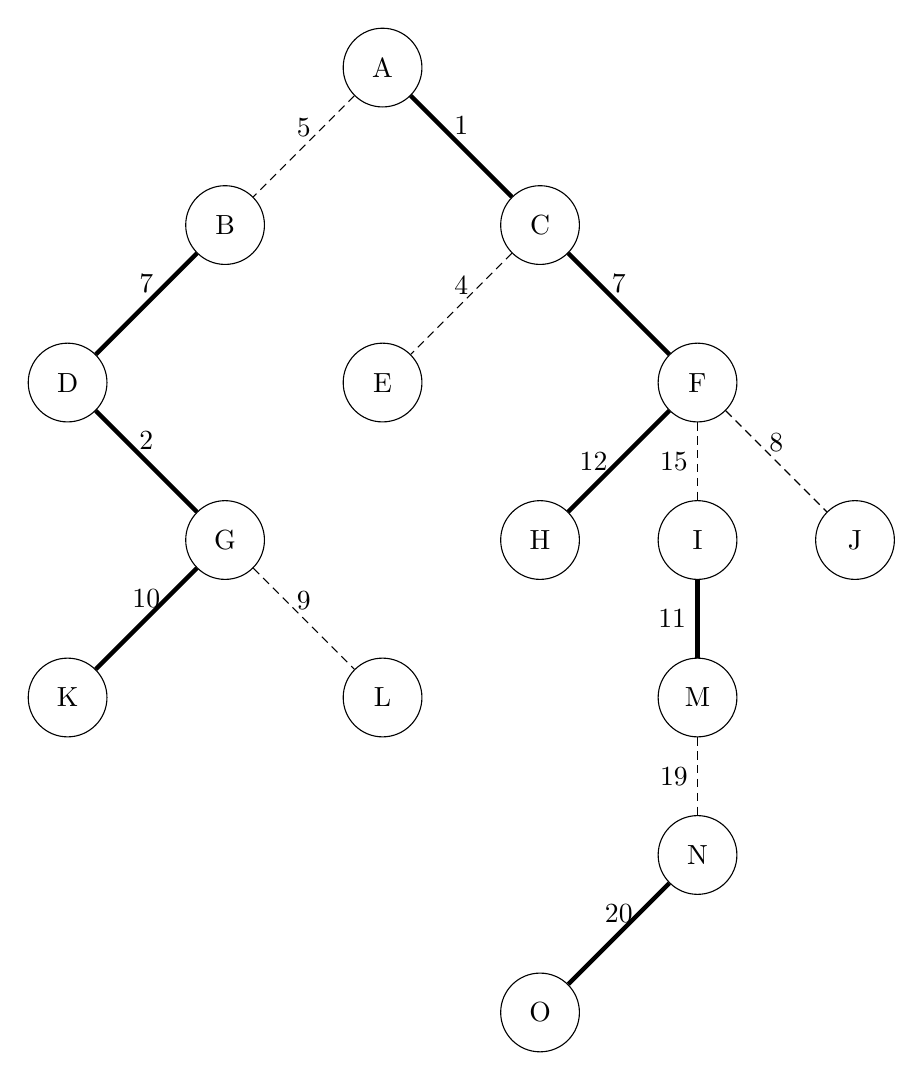
\begin{tikzpicture}[
            nointerno/.style={shape=circle, draw=black, minimum size=1cm},
            pref/.style={ultra thick},
            pptr/.style={densely dashed},
        ]
        \node[nointerno] (a) at (6, 20) {A};
        \node[nointerno] (b) at (4, 18) {B};
        \node[nointerno] (c) at (8, 18) {C};
        \node[nointerno] (d) at (2, 16) {D};
        \node[nointerno] (e) at (6, 16) {E};
        \node[nointerno] (f) at (10, 16) {F};
        \node[nointerno] (g) at (4, 14) {G};
        \node[nointerno] (h) at (8, 14) {H};
        \node[nointerno] (i) at (10, 14) {I};
        \node[nointerno] (j) at (12, 14) {J};
        \node[nointerno] (k) at (2, 12) {K};
        \node[nointerno] (l) at (6, 12) {L};
        \node[nointerno] (m) at (10, 12) {M};
        \node[nointerno] (n) at (10, 10) {N};
        \node[nointerno] (o) at (8, 8) {O};

        \draw[pptr] (a) -- (b) node[midway, above] {5};
        \draw[pref] (a) -- (c) node[midway, above] {1};
        \draw[pref] (b) -- (d) node[midway, above] {7};
        \draw[pref] (d) -- (g) node[midway, above] {2};
        \draw[pref] (g) -- (k) node[midway, above] {10};
        \draw[pptr] (g) -- (l) node[midway, above] {9};
        \draw[pref] (c) -- (f) node[midway, above] {7};
        \draw[pptr] (c) -- (e) node[midway, above] {4};
        \draw[pref] (f) -- (h) node[midway, left] {12};
        \draw[pptr] (f) -- (i) node[midway, left] {15};
        \draw[pptr] (f) -- (j) node[midway, above] {8};
        \draw[pref] (i) -- (m) node[midway, left] {11};
        \draw[pptr] (m) -- (n) node[midway, left] {19};
        \draw[pref] (n) -- (o) node[midway, above] {20};

    \end{tikzpicture}
    \caption{Caminhos preferidos na árvore da Figura \ref{fig:arvore-simples} após uma operação de \texttt{access} no vértice $H$. Com isso temos o novo conjunto de caminhos vértice-disjuntos $ \{ \langle H,F,C,A \rangle, \langle K,G,D,B \rangle, \langle M,I \rangle, \langle E \rangle, \langle J \rangle, \langle L \rangle, \langle O,N \rangle \} $. }
    \label{fig:arvore-access}
\end{figure}

\subsection{Rotinas Make Root, Link e Cut}
\label{subsection:lct-make-root}

Em seguida, temos a função \texttt{make\_root(u)}, que enraíza em $u$ a árvore representada que o contém. Para isso, criamos um caminho preferencial que vai de $u$ até a raiz dessa árvore, utilizando \texttt{access(u)}. Em seguida, utilizamos a rotina \texttt{reverse\_path(u)}, que inverte a orientação deste caminho preferido recém-criado. Tal inversão coloca $u$ como o vértice de menor profundidade da sua árvore representada, o que se traduz neste sendo a nova raiz.

\begin{algorithm}[h!]
    \caption{Rotina Make Root}\label{lct:make-root}
    \begin{algorithmic}[1]
        \Function{make\_root}{{u}}
        \State {access(u)}
        \State {reverse\_path(u)}
        \EndFunction
    \end{algorithmic}
\end{algorithm}

Como rotinas que dão nome à estrutura, temos \texttt{link(u, v, w)} e \texttt{cut(u, v)}.

A primeira delas recebe dois nós $u$ e $v$ que estão em árvores distintas, e cria uma aresta de peso $w$, conectando-os. Primeiramente, devemos lembrar que as arestas da floresta representada viram nós em nossa representação interna. Com isso, o primeiro passo é criar um nó que tem seu valor definido como $w$; vamos chamá-lo \texttt{uv\_edge}. Dessa forma, criaremos as seguintes conexões: $u$ torna-se o pai de \texttt{uv\_edge} e \texttt{uv\_edge} o pai de $v$.

Inicialmente, colocamos $v$ como raiz de sua árvore representada, e criamos um caminho preferido que só possui este vértice como integrante. Com isso, conseguimos concatenar este caminho preferido de tamanho unitário com o caminho que \texttt{uv\_edge} constitui. A seguir, aplicamos a mesma ideia, criando um caminho unitário que contém $u$ em sua árvore e o concatenamos com um caminho que possui $v$ e \texttt{uv\_edge}.

\begin{algorithm}[h!]
    \caption{Rotina Link}\label{lct:link}
    \begin{algorithmic}[1]
        \Require{$u$ e $v$ em árvores distintas}
        \Function{link}{{u, v, w}}
        \State {uv\_edge $\gets$ new Node(w)} \Comment{cria nó com peso $w$, representando a aresta}
        \State \Comment{ligando \emph{(v) - (uv\_edge)}}
        \State {make\_root(v)}
        \State {access(v)}
        \State {join(v, uv\_edge)}
        \State \Comment{ligando \emph{(uv\_edge)-(u)}}
        \State {make\_root(u)}
        \State {access(u)}
        \State {access(uv\_edge)}
        \State {join(uv\_edge, u)}
        \EndFunction
    \end{algorithmic}
\end{algorithm}

Já a operação \texttt{cut(u, v)}, que separa dois vértices ligados por uma aresta, é um pouco mais simples. Note que temos que separar as conexões entre $u$ e \texttt{uv\_edge}, assim como entre \texttt{uv\_edge} e $v$. O processo de separação é igual para as duas partes, por isso vamos explicar somente a separação de $u$ e \texttt{uv\_edge}.

\begin{algorithm}[h!]
    \caption{Rotina Cut}\label{lct:cut}
    \begin{algorithmic}[1]
        \Require{$u$ e $v$ na mesma árvore e $uv$ uma aresta da floresta representada}
        \Function{cut}{{u, v}}
        \State \Comment{cortando \emph{(u) - (uv\_edge)}}
        \State {make\_root(u)}
        \State {access(uv\_edge)}
        \State {split(uv\_edge)}
        \State \Comment{cortando \emph{(v) - (uv\_edge)}}
        \State {make\_root(v)}
        \State {access(uv\_edge)}
        \State {split(uv\_edge)}
        \EndFunction
    \end{algorithmic}
\end{algorithm}

A ideia é colocarmos $u$ como raiz de nossa árvore representada. Com isso, podemos criar um caminho preferido que vai de \texttt{uv\_edge} até $u$ . Agora, basta usarmos nossa operação \texttt{split(uv\_edge)}, que separa \texttt{uv\_edge} da parte superior de seu caminho preferido, efetivamente quebrando sua conexão com $u$.

\subsection{Consultas Is Connected e Maximum Edge}
\label{subsection:lct-is-connected}

A função \texttt{is\_connected(u, v)}, que nos informa se $u$ e $v$ pertencem à mesma árvore, funciona da seguinte maneira. Primeiro acessamos $u$, criando um caminho deste até a raiz da sua árvore. Em seguida, guardamos o vértice que está no fim desse caminho, isto é, guardamos a raiz da árvore que contém $u$. A seguir, repetimos o mesmo processo com o vértice $v$. Agora, basta compararmos se ambos os valores que guardamos são iguais.

\begin{algorithm}[h!]
    \caption{Consulta Is Connected}\label{lct:is-connected}
    \begin{algorithmic}[1]
        \Function{is\_connected}{{u, v}}
        \State {access(u)}
        \State {u\_tree\_root $\gets$ get\_path\_end\_node(u)}
        \State {access(v)}
        \State {v\_tree\_root $\gets$ get\_path\_end\_node(v)}
        \State \Return {(u\_tree\_root = v\_tree\_root)}
        \EndFunction
    \end{algorithmic}
\end{algorithm}

Por último, temos a função \texttt{maximum\_edge(u, v)}, que supõe que $u$ e $v$ estão na mesma árvore da floresta representada e retorna o peso da maior aresta no caminho simples entre $u$ e $v$. Como transformamos as arestas em vértices na nossa representação interna, precisamos procurar o maior valor de um vértice no caminho preferido entre $u$ e $v$. Para isso, transformamos $v$ na raiz de nossa árvore e acessamos $u$. Com isso, podemos utilizar a rotina \texttt{get\_maximum\_path\_value(u)} para obter o maior valor contido neste caminho preferido.

\begin{algorithm}[h!]
    \caption{Consulta Maximum Edge}\label{lct:max-edge}
    \begin{algorithmic}[1]
        \Require{$u$ e $v$ na mesma árvore}
        \Function{maximum\_edge}{{u, v}}
        \State {make\_root(v)}
        \State {access(u)}
        \State \Return {get\_maximum\_path\_value(u)}
        \EndFunction
    \end{algorithmic}
\end{algorithm}

Assim, encerramos a explicação da implementação dos métodos das link-cut trees. Além disso, podemos perceber que todos os métodos executam simplesmente chamadas para os modificadores de caminhos preferidos e para a rotina \texttt{access}. Portanto, temos que as funções apresentadas até agora consomem tempo amortizado $\Oh(\log n)$.

%% ------------------------------------------------------------------------- %%
%% ------------------------------------------------------------------------- %%
%% ------------------------------------------------------------------------- %%
%% ------------------------------------------------------------------------- %%
\section{Splay Trees}
\label{sec:lct-splay-trees}

No artigo original, \citet{10.1145/800076.802464} propuseram a utilização de uma árvore binária enviesada como estrutura para os caminhos preferidos. Porém, quatro anos depois, eles apresentaram a \emph{splay tree} --- \citet{10.1145/3828.3835}, que possibilita realizarmos as operações necessárias para a manipulação dos caminhos preferidos em tempo $\Oh(\log n)$ amortizado, onde $n$ é o número de nós da floresta representada, com uma implementação muito mais elegante do que a da versão original. Portanto, usaremos as splay trees para armazenar os caminhos preferidos.

Uma splay tree é uma árvore binária de busca auto-balanceável. Estas árvores utilizam rotações para se auto-balancear, através de uma operação chamada \texttt{splay}. A operação \texttt{splay} traz um nó para a raiz da árvore através de sucessivas rotações. Mas antes de nos aprofundarmos neste método, examinaremos como os caminhos preferidos são representados aqui.

Primeiramente, em nosso uso, a ordenação dos nós na splay tree é dada pela profundidade destes nas link-cut trees. Note que, para garantir a eficiência, não guardamos explicitamente esses valores. Em vez disso, utilizamos a ideia de chave implícita, isto é, só nos preocupamos em manter a ordem relativa dos nós após as operações de separação e união das árvores, apresentadas a seguir.

Ademais, para implementar eficientemente a operação \texttt{get\_maximum\_path\_value}, mantemos o peso máximo dos nós em cada sub-árvore de uma splay tree.

\begin{figure}
    \centering
    \begin{tikzpicture}[
            no/.style={shape=circle, draw=black, minimum size=1cm},
            novertice/.style={shape=rectangle, draw=black, minimum size=1cm},
            aresta/.style={thick},
        ]
        \node[no] (f) at (6, 10) {F};
        \node[novertice] (ac) at (4, 8) {\shortstack{AC\\$1$}};
        \node[novertice] (fh) at (8, 8) {\shortstack{FH\\$12$}};
        \node[no] (a) at (2, 6) {A};
        \node[no] (c) at (6, 6) {C};
        \node[no] (h) at (10, 6) {H};
        \node[novertice] (cf) at (8, 4) {\shortstack{CF\\$7$}};

        \draw[aresta] (f) -- (ac);
        \draw[aresta] (f) -- (fh);
        \draw[aresta] (ac) -- (a);
        \draw[aresta] (ac) -- (c);
        \draw[aresta] (c) -- (cf);
        \draw[aresta] (fh) -- (h);

    \end{tikzpicture}
    \caption{Uma possível configuração da splay tree que armazena o caminho preferido $\langle H,F,C,A \rangle$ da Figura \ref{fig:arvore-access}, onde $F$ é o identificador do caminho. Os nós em formato retangular mostram as arestas da árvore representada, com o peso de tal aresta na parte inferior.}
    \label{fig:splay-path}
\end{figure}

Além disso, como usamos a profundidade dos nós na árvore representada como chave para a splay tree, temos que todos os nós na sub-árvore esquerda da raiz têm uma profundidade menor que a raiz, enquanto os nós à direita têm uma profundidade maior. Contudo, ao realizamos uma operação \texttt{make\_root(u)}, fazemos com que todos os nós que estavam acima de $u$ na árvore representada se tornem parte de sua sub-árvore. Para isso, incluímos na splay tree um mecanismo para inverter a ordem de todos os seus nós, efetivamente invertendo a orientação de um caminho preferido.

Com isso, os nós da splay tree têm os seguintes campos:

\begin{itemize}
    \item \texttt{parent}: apontador para o pai na splay tree.
    \item \texttt{left\_child} e \texttt{right\_child}: apontadores para os filhos esquerdo e direito de um nó na splay tree.
    \item \texttt{value}: se o nó representa uma aresta da árvore representada guarda o peso desta aresta, senão guarda 0.
    \item \texttt{max\_subtree\_value}: guarda o valor máximo armazenado na sub-árvore do nó.
    \item \texttt{is\_reversed}: valor booleano para sinalizar se a sub-árvore do nó está com sua ordem invertida ou não, isto é, se todas as posições de filhos esquerdos e direitos estão invertidas nessa sub-árvore. Seu funcionamento é ilustrado na Figura \ref{fig:is-reversed-show}.
\end{itemize}

\begin{figure}
    \centering
    \begin{subfigure}[b]{0.7\textwidth}
        \centering
        \begin{tikzpicture}[
                no/.style={shape=circle, draw=black, minimum size=1cm},
                aresta/.style={thick},
            ]
            \node[no, label={0}] (a) at (4, 2) {A};
            \node[no, label={1}] (b) at (6, 4) {B};
            \node[no, label={0}] (c) at (8, 2) {C};
            \node[no, label={1}] (d) at (4, 6) {D};
            \node[no, label={0}] (e) at (2, 4) {E};
            \node[no, label={0}] (g) at (0, 2) {G};
            \node[no, label={0}] (f) at (2, 0) {F};

            \draw[aresta] (d) -- (e);
            \draw[aresta] (d) -- (b);
            \draw[aresta] (b) -- (c);
            \draw[aresta] (b) -- (a);
            \draw[aresta] (e) -- (g);
            \draw[aresta] (f) -- (g);
        \end{tikzpicture}
        \caption{splay tree com valores \texttt{is\_reversed}}
    \end{subfigure}
    \par\bigskip
    \begin{subfigure}[b]{0.7\textwidth}
        \centering
        \begin{tikzpicture}[
                no/.style={shape=circle, draw=black, minimum size=1cm},
                aresta/.style={thick},
            ]
            \node[no] (a) at (0, 2) {A};
            \node[no] (b) at (2, 4) {B};
            \node[no] (c) at (4, 2) {C};
            \node[no] (d) at (4, 6) {D};
            \node[no] (e) at (6, 4) {E};
            \node[no] (f) at (6, 0) {F};
            \node[no] (g) at (8, 2) {G};

            \draw[aresta] (d) -- (e);
            \draw[aresta] (d) -- (b);
            \draw[aresta] (b) -- (c);
            \draw[aresta] (b) -- (a);
            \draw[aresta] (e) -- (g);
            \draw[aresta] (f) -- (g);
        \end{tikzpicture}
        \caption{splay tree após a propagação de todos os valores \texttt{is\_reversed}}
    \end{subfigure}
    \caption{A árvore em (a) mostra os valores do booleano \texttt{is\_reversed} acima do rótulo de cada nó. Já a árvore em (b) mostra a splay tree resultante após todas as inversões serem aplicadas.}
    \label{fig:is-reversed-show}
\end{figure}

Ademais, caso o nó seja a raiz da splay tree, o campo \texttt{parent} armazena um ponteiro para o nó que está logo acima do fim deste caminho preferido na árvore representada. Ou seja, a raiz de uma splay tree aponta para um nó de outra splay tree, aquela que contém o vértice a que seu caminho preferencial se liga na sua árvore representada.

\subsection{Rotina Splay}
\label{subsection:lct-splay-splay}

A rotina \texttt{splay} é o que garante o auto-balanceamento de uma splay tree. Como já mencionamos, seu efeito é trazer um dado nó para a raiz da árvore por meio de uma série de rotações. Para que o custo total de $m$ operações em uma splay com $n$ nós seja $\Oh (m \log n) $, resultando num custo $\Oh(\log n)$ amortizado por operação, a implementação deve garantir que o método \texttt{splay} seja sempre acionado no nó acessado mais profundo da splay tree, em toda operação. Ademais, as rotações que trazem o nó para a raiz da árvore devem seguir uma ordem particular, descrita através dos \emph{passos de splay}, que aplicam rotações duplas ou unitárias, até que o nó em que estamos aplicando a operação chegue à raiz. Por último, devido ao bit que indica a inversão da sub-árvore de cada nó, temos que tomar alguns cuidados extras na nossa implementação dos passos de splay.

Em particular, podemos dizer que esta operação é responsável por transformar um nó em identificador de seu caminho, ou seja, entendemos como sinônimos os métodos \texttt{make\_identifier} e \texttt{splay}.

De modo a facilitarmos nossa explicação detalhada, chamamos de \texttt{parent} o pai de um nó $u$ e de \texttt{grandparent} o pai de \texttt{parent}. Como dissemos, uma operação de \texttt{splay} consiste em realizamos diversos \emph{passos de splay}, que trazem $u$ cada vez mais próximo à raiz da árvore, isto é, em cada um desses passos, realizamos uma ou duas rotações que diminuem a profundidade de $u$. Porém, ao realizar estes passos, temos que nos preocupar com dois fatores:

\begin{itemize}
    \item A propagação do valor booleano $is\_reversed$ de \texttt{grandparent} e em seguida o de \texttt{parent}, fazendo as devidas reversões caso necessário. Isso nos fornece a invariante de que iremos fazer comparações entre os filhos corretos para determinar qual rotação fazer.
    \item A orientação em que \texttt{grandparent}, \texttt{parent} e $u$ se encontram, isto é, se estão em uma orientação que Sleator e Tarjan chamaram de \textit{zig}, \textit{zig-zig} ou \textit{zig-zag}, como exemplificadas na Figura \ref{fig:zig-oris}. Dependendo da orientação, fazemos uma rotação em $u$ ou em \texttt{parent}, sempre com a ideia de diminuirmos em 1 a profundidade de $u$.
\end{itemize}

\begin{figure}[H]
    \centering
    \begin{subfigure}[b]{0.3\textwidth}
        \centering
        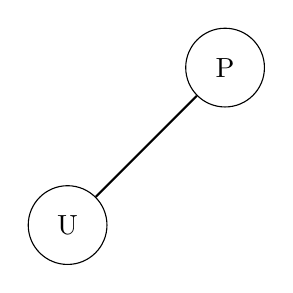
\begin{tikzpicture}[
                no/.style={shape=circle, draw=black, minimum size=1cm},
                aresta/.style={thick},
            ]
            \node[no] (u) at (0, 0) {U};
            \node[no] (p) at (2, 2) {P};
            \draw[aresta] (u) -- (p);
        \end{tikzpicture}
        \caption{zig}
    \end{subfigure}
    \hfill
    \begin{subfigure}[b]{0.3\textwidth}
        \centering
        \begin{tikzpicture}[
                no/.style={shape=circle, draw=black, minimum size=1cm},
                aresta/.style={thick},
            ]
            \node[no] (u) at (0, 0) {U};
            \node[no] (p) at (2, 2) {P};
            \node[no] (gp) at (4, 4) {GP};
            \draw[aresta] (u) -- (p);
            \draw[aresta] (p) -- (gp);
        \end{tikzpicture}
        \caption{zig-zig}
    \end{subfigure}
    \hfill
    \begin{subfigure}[b]{0.3\textwidth}
        \centering
        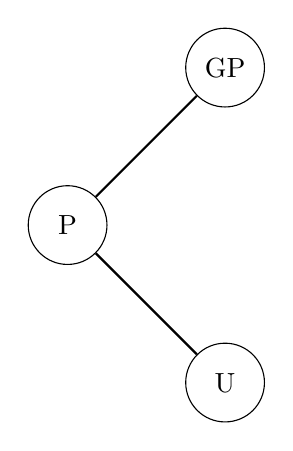
\begin{tikzpicture}[
                no/.style={shape=circle, draw=black, minimum size=1cm},
                aresta/.style={thick},
            ]
            \node[no] (u) at (4, 0) {U};
            \node[no] (p) at (2, 2) {P};
            \node[no] (gp) at (4, 4) {GP};
            \draw[aresta] (u) -- (p);
            \draw[aresta] (p) -- (gp);
        \end{tikzpicture}
        \caption{zig-zag}
    \end{subfigure}
    \caption{Orientações \textit{zig}, \textit{zig-zig} e \textit{zig-zag} na splay tree. Aqui, \texttt{P} e \texttt{GP} abreviam \texttt{parent} e \texttt{grandparent}, respectivamente. As orientações  \textit{zag}, \textit{zag-zag} e \textit{zag-zig} são simétricas a estas.}
    \label{fig:zig-oris}
\end{figure}


Ao sair da função \texttt{splay}, o nó $u$ estará na raiz da splay tree que o contém. Além disso, seu valor booleano $is\_reversed$ estará nulo, pois as reversões já terão sido propagadas aos seus filhos, e seu $max\_subtree\_value$ estará atualizado, contendo o maior valor presente na splay tree.

\begin{algorithm}[h!]
    \caption{Rotina Splay}\label{splay:splay}
    \begin{algorithmic}[1]
        \Function{Splay}{{u}}
        \WhileNot  {{u.is\_root()}} \Comment{$u$ não é raiz da splay tree}
        \State {parent $\gets$ u.parent}
        \State {grandparent $\gets$ parent.parent}
        \IfNot{{parent.is\_root()}}
        \State \Comment{caso o seja necessário, inverte os filhos do nó e propaga a inversão do bit}
        \State {grandparent.push\_reversed\_bit()}
        \State {parent.push\_reversed\_bit()}
        \If{{(grandparent.r\_child = parent) = (parent.r\_child = u)}}
        \State {rotate(parent)} \Comment{zig-zig ou zag-zag}
        \Else
        \State {rotate(u)} \Comment{zig-zag}
        \EndIf
        \EndIf
        \State {rotate(u)}
        \EndWhile
        \State {u.push\_reversed\_bit()}
        \EndFunction
    \end{algorithmic}
\end{algorithm}

Assim como a operação acima, o restante da nossa implementação de uma splay tree é bastante tradicional. Com isso, nossos únicos cuidados extras são a manutenção do bit \texttt{is\_reversed}, do valor máximo das sub-árvores e da consistência das chaves implícitas. Por exemplo, no método \texttt{rotate(u)}, temos como primeiro passo a propagação do bit \texttt{is\_reversed} de \texttt{grandparent} até $u$ e como última etapa o cálculo dos novos valores de \texttt{max\_subtree\_value}.

\subsection{Rotinas Split e Join}
\label{subsection:lct-splay-split-join}

Temos também dois métodos importantes das splay trees usados na manutenção dos caminhos preferidos: \texttt{split} e \texttt{join}, responsáveis por separar e concatenar caminhos preferidos, respectivamente.

Primeiramente, falaremos do método \texttt{split(u)}, que recebe um nó $u$, identificador de seu caminho preferido, e separa o caminho preferido que o contém em dois: um com os nós menos profundos que $u$ em seu caminho, e outro com $u$ e os nós mais profundos que~$u$. Para isso, o método simplesmente separa a sub-árvore esquerda de $u$. Vale notar que este método é destrutivo, removendo tanto o ponteiro para o filho preferido de $u$ quanto o ponteiro \texttt{parent} que tal filho possui para $u$. Logo, usamos essa rotina apenas para o \texttt{cut()} das link-cut trees.

\begin{algorithm}[H]
    \caption{Rotina Split}\label{splay:split}
    \begin{algorithmic}[1]
        \Require{$u$ é identificador de seu caminho preferido}
        \Function{split}{{u}}
        \If{{u.l\_child $\neq$ NULL}}
        \State {u.l\_child.parent $\gets$ NULL}
        \EndIf
        \State {u.l\_child $\gets$ NULL}
        \EndFunction
    \end{algorithmic}
\end{algorithm}

De maneira complementar, temos a rotina \texttt{join(u, v)}, que recebe dois nós e concatena a parte superior do caminho preferido de $u$ ao caminho preferido de $v$. Para isso, assume-se que $v$ seja filho de $u$ na árvore representada que os contém, além de que ambos os nós sejam identificadores de seus caminhos preferidos, ou seja, que eles sejam as raízes de suas splay trees. Com isso, simplesmente colocamos a splay tree em que $v$ é raiz como a sub-árvore direita de $u$, atualizando os respetivos apontadores e recalculando o valor máximo na splay tree de $u$.

\begin{algorithm}[h!]
    \caption{Rotina Join}\label{splay:join}
    \begin{algorithmic}[1]
        \Require{$u$ e $v$ são identificadores de seus caminhos preferidos}
        \Function{join}{{u, v}}
        \If{{v $\neq$ NULL}}
        \State {v.parent $\gets$ u}
        \EndIf
        \State {u.r\_child $\gets$ v}
        \State \Comment{atualiza \texttt{max\_subtree\_value} com o máximo entre o \texttt{value} dos dois filhos de $u$}
        \State {u.recalculate\_max\_subtree\_value()}
        \EndFunction
    \end{algorithmic}
\end{algorithm}

Note que o vértice $u$ poderia ter uma sub-árvore direita, correspondendo à parte mais profunda de seu caminho preferido. Após a operação \texttt{join}, esse trecho de seu velho caminho preferido torna-se um novo caminho preferido que aponta --- através do ponteiro \texttt{parent} --- para o novo caminho preferido de $u$, que acabou de ser concatenado ao de~$v$.

Como ambas as rotinas simplesmente leem e alteram variáveis, definimos seus respectivos custos como $\Oh(1)$.

\subsection{Métodos auxiliares}
\label{subsection:lct-splay-aux}

Para finalizar, nossa splay tree possui quatro métodos auxiliares: o \texttt{reverse\_path}, \texttt{get\_path\_end\_node}, \texttt{get\_parent\_path\_node} e \texttt{get\_maximum\_path\_value}.

Primeiramente, o \texttt{reverse\_path(u)} recebe o identificador $u$ de um caminho e inverte a orientação desse caminho. Tal tarefa é realizada invertendo o valor do bit \texttt{is\_reversed} de $u$. Com isso, nas próximas operações realizadas neste nó, seus filhos serão trocados de posição e o bit será propagado nas suas sub-árvores. Além disso, podemos perceber que seu custo é $\Oh(1)$.

\begin{algorithm}[h!]
    \caption{Rotina Revese Path}\label{splay:reverse-path}
    \begin{algorithmic}[1]
        \Require{$u$ identificador de seu caminho preferido}
        \Function{revese\_path}{{u}}
        \State {u.is\_reversed $\gets$ \textbf{not} u.is\_reversed}
        % \State {u.push\_reversed\_bit()} \Comment{inverte os filhos de $u$ e propaga a inversão do bit}
        \EndFunction
    \end{algorithmic}
\end{algorithm}

A seguir, os métodos \texttt{get\_path\_end\_node(u)} e \texttt{get\_parent\_path\_node(u)} são usados para acessar o fim e o pai do caminho preferido que contém $u$. Em particular, a primeira rotina retorna o nó menos profundo do caminho preferido de $u$, fazendo isso ao acessar o nó mais à esquerda na sua splay tree. Já o segundo método é responsável por retornar o nó imediatamente acima do fim do caminho preferido que contém $u$. Caso tal caminho contenha a raiz da árvore representada, este método retorna \texttt{null}. Para fazer isso, efetuamos uma operação \texttt{splay} em $u$ e retornamos o valor de seu \texttt{parent}.

\begin{algorithm}[h!]
    \caption{Consulta Get Path End Node}\label{splay:get-path-end}
    \begin{algorithmic}[1]
        \Function{get\_path\_end\_node}{{u}}
        \State {splay(u)}
        \State {smallest\_value $\gets$ u}
        \While{{smallest\_value.l\_child $\neq$ NULL}}
        \State {smallest\_value $\gets$ smallest\_value.l\_child}
        \EndWhile
        \State {splay(smallest\_value)}
        \State \Return {smallest\_value}
        \EndFunction
    \end{algorithmic}
\end{algorithm}

\begin{algorithm}[h!]
    \caption{Consulta Get Parent Path Node}\label{splay:get-parent-path}
    \begin{algorithmic}[1]
        \Function{get\_parent\_path\_node}{{u}}
        \State {splay(u)}
        \State \Return {u.parent}
        \EndFunction
    \end{algorithmic}
\end{algorithm}

Como as duas rotinas acima utilizam o método \texttt{splay}, podemos afirma que os respectivos custos são de $\Oh(\log n)$ amortizado.

Por último, temos a função \texttt{get\_maximum\_path\_value(u)}, que recebe um nó $u$ identificador de caminho e retorna o maior valor de uma aresta no caminho preferencial de $u$. Em termos práticos, retorna o valor de \texttt{max\_subtree\_value}. Claramente, temos que o custo de tal função é $\Oh(1)$.

\begin{algorithm}[h!]
    \caption{Consulta Get Maximum Path Value}\label{splay:get-maximum-value}
    \begin{algorithmic}[1]
        \Require{$u$ identificador de seu caminho preferido}
        \Function{get\_maximum\_path\_value}{{u}}
        \State \Return {u.max\_subtree\_value}
        \EndFunction
    \end{algorithmic}
\end{algorithm}

Com isso, temos todas as ferramentas necessárias para manipularmos a splay tree em seu uso representando os caminhos preferidos nas link-cut trees.